\chapter{Introduction}
In recent years, advancements in computer vision technology and hardware for mobile devices
have enabled the development of mobile applications that can understand and interact with the real world.
Augmented Reality (AR) is a popular application of this technology,
allowing for the overlay of digital information onto the real world.
For instance, in the ecommerce industry, companies like Amazon are leveraging AR to
enable customers to visualize furniture in their homes before making a purchase.
Similarly, mobile mapping applications utilize AR to provide directions and information about the
environment through the camera feed.

Virtual Reality (VR) on the other hand creates fully immersive experiences
that isolate users from the real world.
Through the use of specialized head-mounted display (HMD) headsets, users can explore virtual worlds,
play games, and watch movies in environments completely separate from their physical surroundings.
This technology has gained traction in the gaming and entertainment industries
with platforms like Oculus Rift, SteamVR and PlayStation VR.

Building upon the advancements of VR and mobile AR,
a recent trend in the industry is the development of devices that combine the two technologies,
allowing to seamlessly blend virtual objects into the real world and vice versa, creating the illusion of a singular, unified world.
This technology is named differently by different companies, such as Mixed Reality (MR) by Microsoft and Meta
or Spatial Computing by Apple.
MR / Spatial Computing allows for immersive experiences while still enabling users to interact with the real world.
Similarly to AR, its potential applications span across various industries, from healthcare to education to entertainment.
Examples of devices include Microsoft's HoloLens and more recently the Meta Quest 3 and Apple Vision Pro.

Figure~\ref{fig:quest3-example} shows a screenshot of a trailer for a game on the Quest 3 that mixes the real world with virtual objects.
You can see virtual boxes and enemies blended into the real environment of the player.
The player can interact with these objects with their body and hands, using controllers or hand tracking.
%Figure~\ref{fig:visonpro-example} shows a screenshot of the Apple Vision Pro bing used in a professional setting.
%You can see a person using the device to work on virtual screen while being in a video call with colleagues,
%all while being in their real environment.

%\begin{figure}[ht!]
%    \centering
%    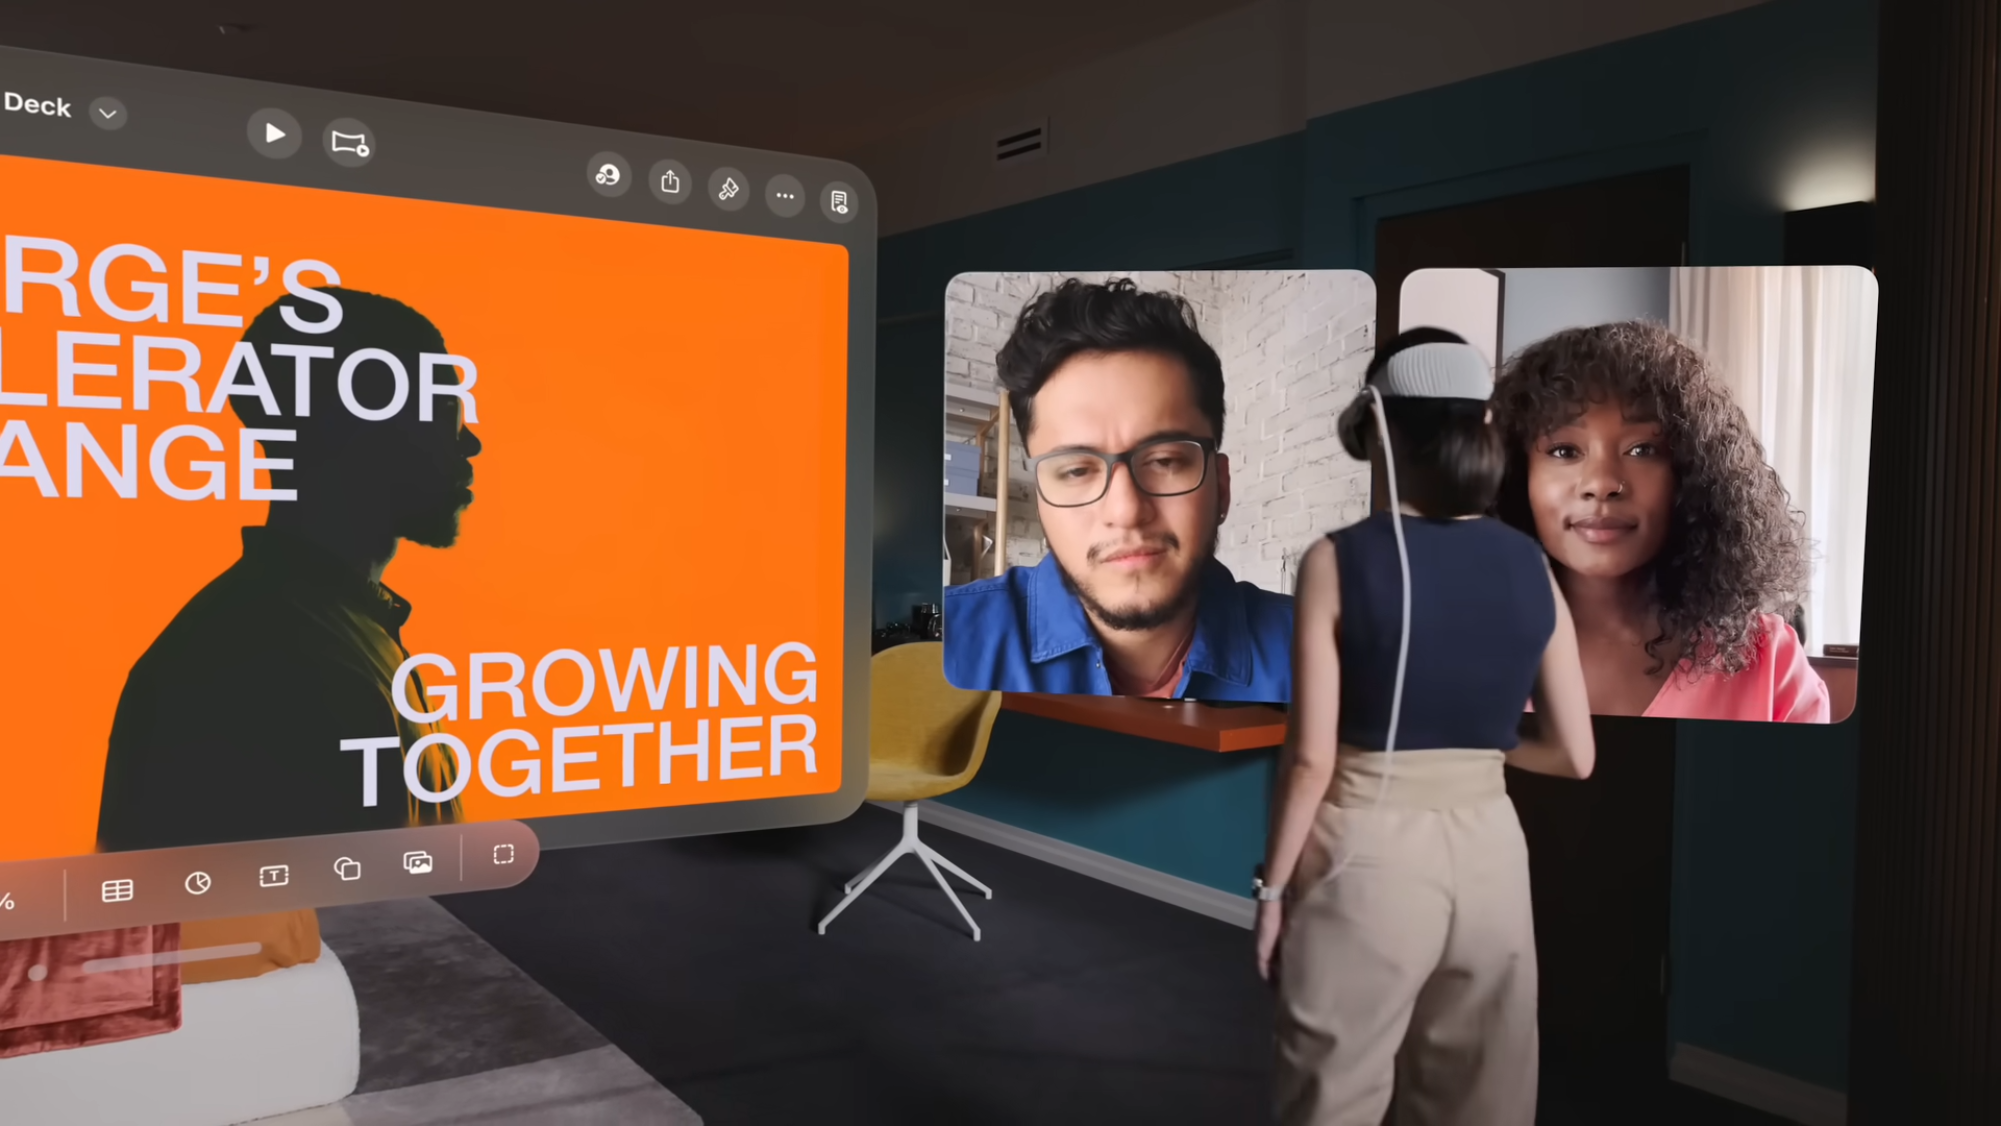
\includegraphics[width=0.8\linewidth]{images/Apple - Introducing Apple Vision Pro [TX9qSaGXFyg - 2001x1126 - 4m41s]}
%    \caption{Screenshot of the Apple Vision Pro announcement video at Apple Worldwide Developers Conference 2023 showcasing the device for professional use-cases.}
%    \label{fig:visonpro-example}
%\end{figure}
%
Current AR applications use a variety of techniques to blend virtual objects into the real world and make them interactable.
As an example, the ARCore Depth SDK by Google provides features like
\begin{itemize}
    \item Detection of flat surfaces
    \item Placement of virtual objects on surfaces
    \item Depth information that can be used to occlude objects behind real-world objects
    \item Lighting estimation for realistic shading of virtual objects
\end{itemize}
This however, does not allow for understanding of the environment for the purpose of complex logic outside of rendering,
such as navigation of AI agents through the environment or creating customized game logic based on the layout of the environment,
as the API does not provide a mesh of the environment or similar features.
To enable these kinds of applications, it is essential to have an accurate understanding of the real world surrounding the user.

This thesis aims to provide an implementation of a system that can create a mesh of the environment
from data provided by the ARCore Depth API using primitive detection algorithms and overlay this mesh onto the camera feed for visualization.
The information about the environment (both the primitive parameterization and the resulting mesh) can then be used for various applications as mentioned above.
\begin{figure}[h]
    \centering
    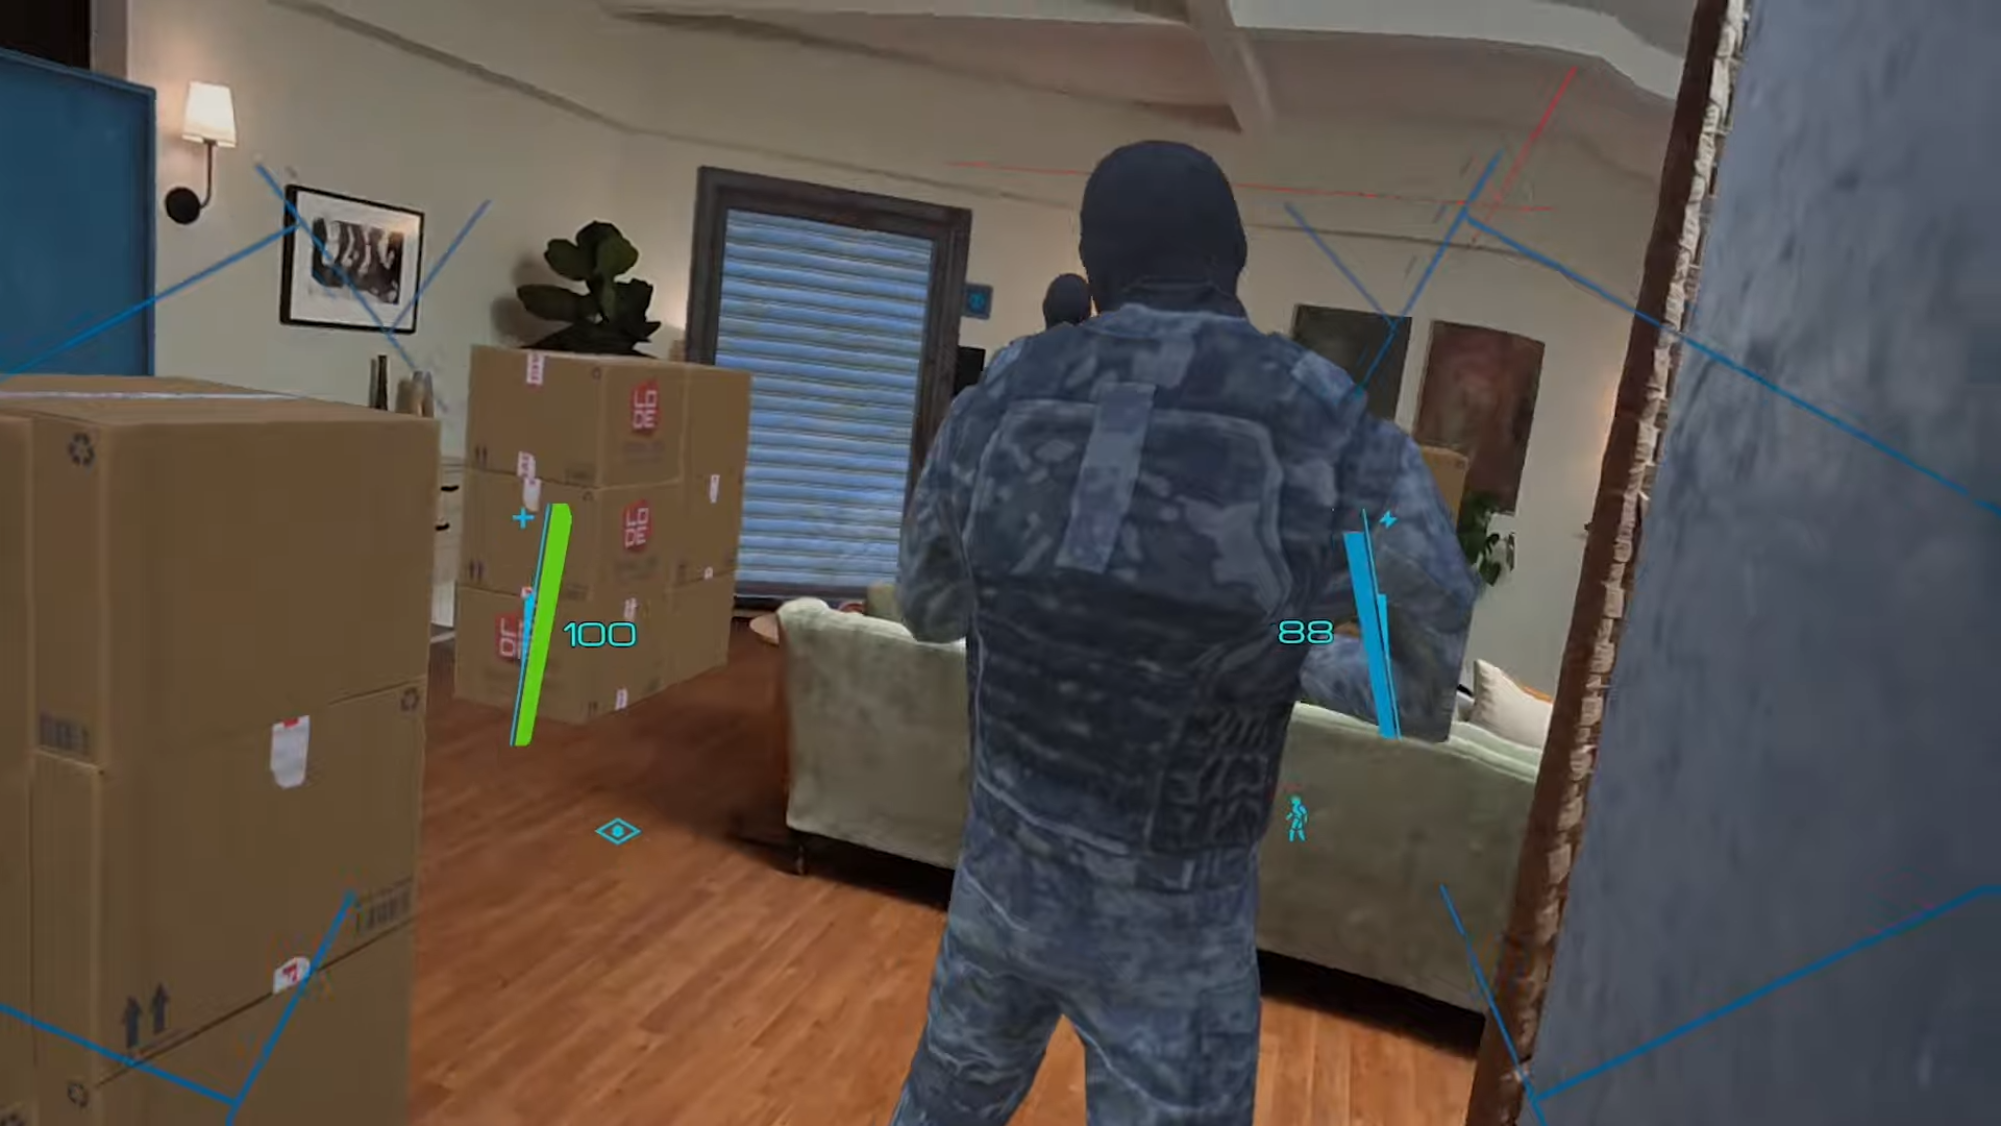
\includegraphics[width=0.8\linewidth]{images/Tripwire Interactive - Espire 2 Mixed Reality Update Trailer [50DD3XwjOIA - 2001x1126 - 0m21s]}
    \caption{Screenshot of trailer for the game Espire 2 by Tripwire Interactive showcasing a player using the Meta Quest 3 playing the game blended with their real environment.}
    \label{fig:quest3-example}
\end{figure}


%\section{Research Aims}
%Object detection and classification are fundamental problems of both Augmented Reality (AR) and computer vision.

%The following questions are under consideration.
%\begin{enumerate}
%    \item What is the nature of the objects to be detected? Should the items be geometric primitives themselves, or should more complex items be approximated using geometric primitives?
%    \item How should the selection of objects for tracking be determined? Should the algorithm autonomously identify the most suitable approximation, or should the process be guided by user interaction, such as selecting an object on the screen to initiate detection?
%    \item Should multiple objects be detected at the same time?
%    \item Should the objects be tracked? If yes, under which conditions? Should tracking occur:
%    \begin{enumerate}
%        \item while the device is in motion,
%        \item while the object itself is in motion, or
%        \item under a combination of both conditions?
%    \end{enumerate}
%    \item Should the detection be reevaluated as new data arrives?
%    \item Which assumptions can be made about the environment?
%\end{enumerate}
%



%\subsection{Augmented Reality, Virtual Realtiy and Mixed Reality}
%
%\subsection{Trends in the industry}
%
%\section{Related Work}
